\documentclass[a4paper,11pt]{article}
\usepackage{amsmath,amsthm,amsfonts,amssymb,amscd,amstext,vmargin,graphics,graphicx,tabularx,multicol} \usepackage[french]{babel}
\usepackage[utf8]{inputenc}  
\usepackage[T1]{fontenc} 
\usepackage[T1]{fontenc}
\usepackage{amsmath,amssymb}
\usepackage{pstricks-add,tikz,tkz-tab,variations}
\usepackage[autolanguage,np]{numprint} 

\setmarginsrb{1.5cm}{0.5cm}{1cm}{0.5cm}{0cm}{0cm}{0cm}{0cm} %Gauche, haut, droite, haut
\newcounter{numexo}
\newcommand{\exo}[1]{\stepcounter{numexo}\noindent{\bf Exercice~\thenumexo} : \marginpar{\hfill /#1}}
\reversemarginpar


\newcounter{enumtabi}
\newcounter{enumtaba}
\newcommand{\q}{\stepcounter{enumtabi} \theenumtabi.  }
\newcommand{\qa}{\stepcounter{enumtaba} (\alph{enumtaba}) }
\newcommand{\initq}{\setcounter{enumtabi}{0}}
\newcommand{\initqa}{\setcounter{enumtaba}{0}}

\newcommand{\be}{\begin{enumerate}}
\newcommand{\ee}{\end{enumerate}}
\newcommand{\bi}{\begin{itemize}}
\newcommand{\ei}{\end{itemize}}
\newcommand{\bp}{\begin{pspicture*}}
\newcommand{\ep}{\end{pspicture*}}
\newcommand{\bt}{\begin{tabular}}
\newcommand{\et}{\end{tabular}}
\renewcommand{\tabularxcolumn}[1]{>{\centering}m{#1}} %(colonne m{} centrée, au lieu de p par défault) 
\newcommand{\tnl}{\tabularnewline}

\newcommand{\trait}{\noindent \rule{\linewidth}{0.2mm}}
\newcommand{\hs}[1]{\hspace{#1}}
\newcommand{\vs}[1]{\vspace{#1}}

\newcommand{\N}{\mathbb{N}}
\newcommand{\Z}{\mathbb{Z}}
\newcommand{\R}{\mathbb{R}}
\newcommand{\C}{\mathbb{C}}
\newcommand{\Dcal}{\mathcal{D}}
\newcommand{\Ccal}{\mathcal{C}}
\newcommand{\mc}{\mathcal}

\newcommand{\vect}[1]{\overrightarrow{#1}}
\newcommand{\ds}{\displaystyle}
\newcommand{\eq}{\quad \Leftrightarrow \quad}
\newcommand{\vecti}{\vec{\imath}}
\newcommand{\vectj}{\vec{\jmath}}
\newcommand{\Oij}{(O;\vec{\imath}, \vec{\jmath})}
\newcommand{\OIJ}{(O;I,J)}

\newcommand{\bmul}[1]{\begin{multicols}{#1}}
\newcommand{\emul}{\end{multicols}}


\newcommand{\reponse}[1][1]{%
\multido{}{#1}{\makebox[\linewidth]{\rule[0pt]{0pt}{20pt}\dotfill}
}}

\newcommand{\titre}[5] 
% #1: titre #2: haut gauche #3: bas gauche #4: haut droite #5: bas droite
{
\noindent #2 \hfill #4 \\
#3 \hfill #5

\vspace{-1.6cm}

\begin{center}\rule{6cm}{0.5mm}\end{center}
\vspace{0.2cm}
\begin{center}{\large{\textbf{#1}}}\end{center}
\begin{center}\rule{6cm}{0.5mm}\end{center}
}



\begin{document}
\pagestyle{empty}
\titre{Devoir maison 1 }{Nom :}{Prénom :}{Classe}{Date}

\vspace*{0.2cm}

\exo{3} Construire le symétrique de chacune de ces figures par rapport au point marqué.\\


\includegraphics[scale=0.8]{symcen1.eps} \hspace*{2cm}\includegraphics[scale=0.8]{symcen2.eps} \\


\exo{3} Construire le symétrique de chacune de ces figures par rapport au point marqué.\\

\hspace*{2.5cm}\includegraphics[scale=0.8]{symcen4.eps} 


\hspace*{1cm} 
\includegraphics[scale=0.8]{symcen3.eps}

\newpage

\vspace*{0.2cm}

\exo{4} Calculer les expressions suivantes et donner votre réponse sous forme de fraction irréductible. \\

\bmul{2}

$P = \dfrac{4}{9} - \dfrac{1}{9} + \dfrac{18}{9}$\\



$K =  \dfrac{1}{7} + \dfrac{2}{5}$\\

\columnbreak

$A =   \dfrac{7}{6} - \left( \dfrac{11}{30} - \dfrac{3}{15} \right)   $\\



$N = \left(  \dfrac{1}{3} + \dfrac{5}{24}  \right)- \left(  \dfrac{1}{4} + \dfrac{1}{12}\right)$\\

\emul

\vspace*{0.5cm}

\exo{2}\\
Maxime refait la tapisserie de son salon. Il pose $\dfrac{4}{15}$ du papier peint le premier jour,  $\dfrac{2}{5}$ le deuxième jour et  $\dfrac{1}{6}$ le troisième jour.\\

Aura-t-il terminé le troisième jour ? Justifier votre réponse.\\

\vspace*{0.5cm}

\exo{3}\\
Recopier et compléter cette pyramide de sorte à ce que le nombre figurant dans chaque case soit égal à la somme des nombres figurant sur les 2 cases sur lesquelles elle repose.\\ 
Écrire vos calculs sur votre copie.

\begin{center}
\includegraphics[scale=0.4]{pyramide.eps} 
\end{center}





\end{document}
